
\begin{minipage}[c][\textheight][c]{\linewidth}

    \section{Introducción}
    El presente documento tiene como objetivo presentar un algoritmo genético diseñado para abordar una problemática común en el ámbito estudiantil: la selección óptima de materias para un estudiante en un estado de irregularidad académica. Esta herramienta de software propone una solución que determina la distribución más adecuada de materias teniendo en cuenta los grupos disponibles en el cuatrimestre próximo, así como la secuencia recomendada dentro del plan de estudios y el progreso académico del estudiante. La exposición detallada del análisis, la metodología empleada y el desarrollo del software facilita la comprensión de su funcionamiento y su aplicación práctica en el contexto educativo.

\end{minipage}

\newpage

\section{Análisis del Problema}
Para abordar la resolución de la problemática planteada, se llevó a cabo una exhaustiva identificación de los elementos pertinentes que influyen en el funcionamiento del algoritmo, así como su efectiva interpretación numérica para su implementación en un algoritmo genético.

\subsection{Problemática}
El núcleo del problema radica en la necesidad de planificar el horario académico del próximo cuatrimestre para un estudiante, basándose en su historial académico, el cual comprende un conjunto de materias que ha cursado o reprobado, teniendo en cuenta su progreso académico actual. Este desafío implica la evaluación de cada materia según su umbral de relavancia \ref{umbral_relevancia} y siempre evitando el solapamientos de horarios entre las disponibles por grupo. El funcionamiento general del algoritmo puede esquematizarse de la siguiente manera:

\begin{figure}[h]
    \centering
    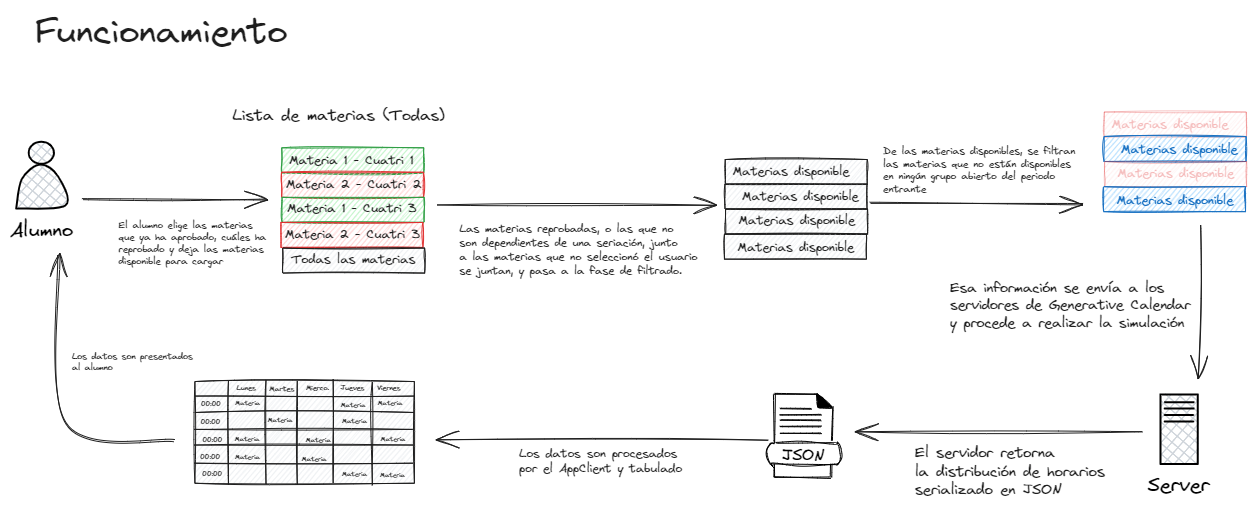
\includegraphics[width=\textwidth]{images/AG-funcionamiento.png}
    \label{Diagrama del funcionamiento general del algoritmo.}
    \caption{Diagrama del funcionamiento general del algoritmo.}
\end{figure}

\section{Resolución de problemas}

En esta sección se describe el enfoque adoptado para abordar el problema y alcanzar los objetivos del programa. La resolución del problema se divide en los siguientes puntos, que se detallarán a través de las diferentes subsecciones del documento.

\begin{enumerate}
    \item Captura de progreso académico. $_{\text{\ref{captura_progreso_académico}}}$
    \item Filtrado de materias por seriación $_{\text{\ref{filtrado_de_materias_por_seriacion}}}$
    \item Filtrado de materias por disponibilidad horaria. $_{\text{\ref{filtrado_de_materias_por_disponibilidad_horaria}}}$
    \item Cuantificación de los datos. $_{\text{\ref{cuantifiacion_de_datos}}}$
    \item Procesamiento de la información. $_{\text{\ref{procesamiento_de_la_informacion}}}$
\end{enumerate}

\subsection{Captura de progreso académico.} \label{captura_progreso_académico}
La primera etapa del proceso del algoritmo se centra en la captura del progreso académico actual del alumno, es decir, las materias cursadas o reprobadas por el alumno. En esta fase, el alumno seleccionará manualmente las materias que ha aprobado y las que ha reprobado, dejando libres aquellas que aún no ha cursado. Esta acción proporciona al sistema un contexto claro sobre el estado y el progreso del alumno. Además, la implementación de la seriación de materias, facilitará el completado y filtrado de las materias \ref{filtrado_de_materias_por_seriacion}. 

\begin{figure}[h]
    \centering
    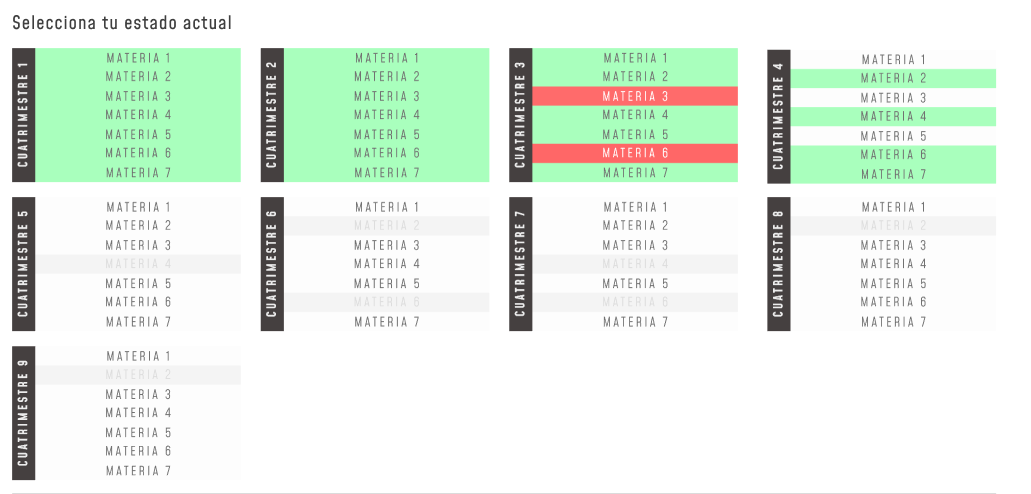
\includegraphics[width=\textwidth]{images/current_status_figma_screenshot.png}
    \caption{Captura de pantalla de la sección de selección de materias cursadas, obtenida del maquetado en Figma.}
    \label{fig:captura_materias}
\end{figure}

\subsection{Filtrado de materias por seriación} \label{filtrado_de_materias_por_seriacion}
El proceso de filtrado de materias tiene como objetivo eliminar aquellas materias que, debido a restricciones de seriación, no deben considerarse como materias aptas para carga. Estas materias, denominadas ``materias aptas para carga", son aquellas que cumplen con sus requerimiento de materias previas, y como consecuencia, pueden ser consideradas aptas para el procesamiento del algoritmo. Es importante destacar que el Algoritmo Genético (AG) procesa únicamente conjuntos de materias de forma individual, sin tener un contexto completo de la seriación o adeudos de materias del alumno, por lo que este paso es importante para generar un horario válido y un funcionamiento correcto. %\\

Una vez que el usuario ha seleccionado las materias aprobadas, estas se guardan en un arreglo de materias \( M \), donde se almacenan todas las materias iniciales \( N \) etiquetadas según la selección del alumno. De esta forma, el arreglo de materias \( M \) se define como: %\\

\begin{equation}
    M : \{ N_1, N_2, \dots, N_i \}
    \label{eq:arreglo_materias_sin_procesar}
\end{equation} \myequations{Arreglo de materias sin procesar.}

\noindent
Donde \( N_i \) es la materia alojada en la posición \( i \) del arreglo \( M \), y se podría definir a \( N_i \) de la siguiente manera: %\\

\begin{equation}
    N_i : (\text{id}_i, \text{name}_i, \text{status}_i, [\text{dependencias}]_i, [\text{dependientes}]_i, \text{cuatrimestre}_i,  \text{peso}_i)
    \label{eq:atributos_materia}
\end{equation} \myequations{Atributos de las asignaturas sin procesar.}

\noindent
Donde cada atributo de los objetos materia obedece las siguientes definiciones:
\begin{itemize}
    \item \( \text{id} \): es el identificador único de la materia conformado por caracteres alfabéticos de longitud 4.
    \item \( \text{name} \): es el nombre común de la materia en cuestión.
    \item \( \text{status} \): es el estado que ha elegido el alumno, que puede ser: aprobado, reprobado, o sin cursar.
    \item \( [\text{dependencias}] \): es un arreglo de longitud \( n \) que contiene todos los identificadores de las materias que se deben cursar antes de poder cursar la materia actual.
    \item \( [\text{dependientes}] \): es un arreglo de todas las materias que dependen de la materia actual, es decir, aquellas materias que se podrán cursar una vez que la materia actual haya sido aprobada.
    \item \( \text{cuatrimestre} \): corresponde a un identificador numérico del 1 al 9, que indica el cuatrimestre regular en el que debería ser cursada dicha materia.
    \item \( \text{peso} \): corresponde a un número entero mayor o igual a 0, que representa la cantidad de materias que dependen de la asignatura actual, ver sección \ref{umbral_relevancia}.
\end{itemize}


\subsubsection{Seriación}

\begin{figure}[h]
    \centering
    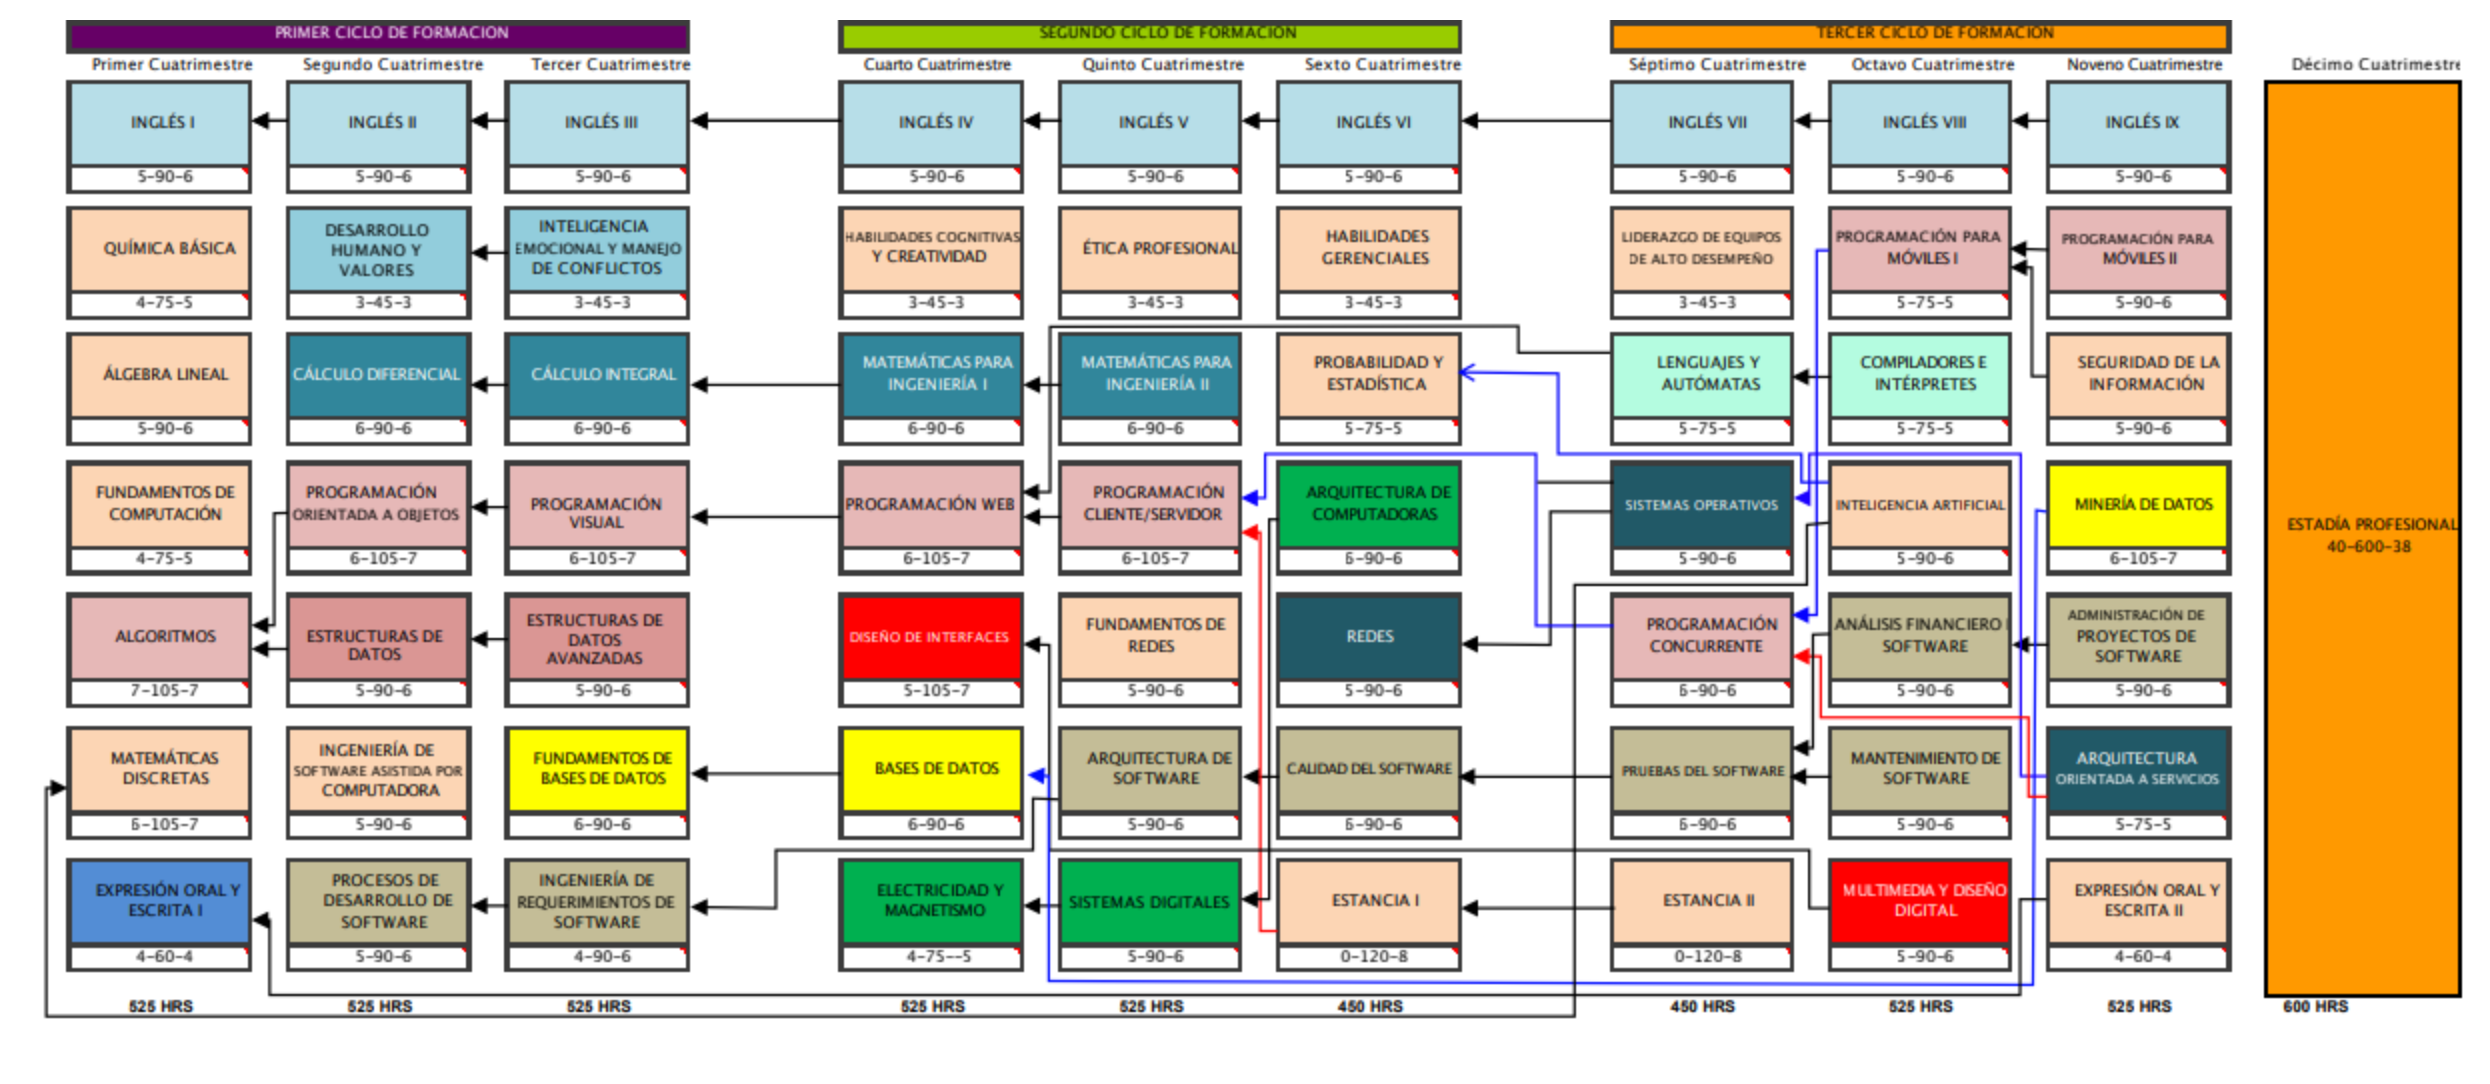
\includegraphics[width=\textwidth]{images/mapa_curricular.png}
    \caption{Mapa curricular de la carrera de Ingeniería en Desarrollo de Software del año 2017.}
    \label{fig:mapa_curricular_ids_2017}
\end{figure}

Es importante destacar que las materias que se maneja internamente en el programa, tienen una lista de materias dependientes y una de materias de dependencias. Esta característica se debe a la seriación, la cual dicta qué materias se podrán cursar en función del progreso del alumno. %\\

La seriación, como es comúnmente conocida, se ajusta al mapa curricular de la carrera para la cual se desarrolló el algoritmo. En el caso actual, dicho mapa curricular corresponde a la carrera de \textbf{Ingeniería en Desarrollo de Software} (IDS). %\\

El algoritmo se basó en el mapa curricular de IDS del año 2017. Como se puede observar en la figura \ref{fig:mapa_curricular_ids_2017}, existen materias que solo se podrán cursar una vez que todas las materias requeridas sean aprobadas. %\\


\subsubsection{Depuración de materias} \label{depuracion_de_materias}
Es fundamental tener en cuenta que existen materias que no pueden ser cursadas hasta que se aprueben una o más asignaturas de su línea de seriación. Por lo tanto, se debe eliminar de la lista de materias todas aquellas asignaturas que, según el caso de cada alumno, no sean aptas para ser cargadas debido a motivos de reprobación o porque su esquema de seriación está incompleto. %\\

Para ilustrar este concepto, consideremos un ejemplo y simplifiquemos el mapa curricular como se muestra en la figura \ref{fig:mapa_curricular_simplificado_caso_1}: %\\

\begin{figure}[h]
    \centering
    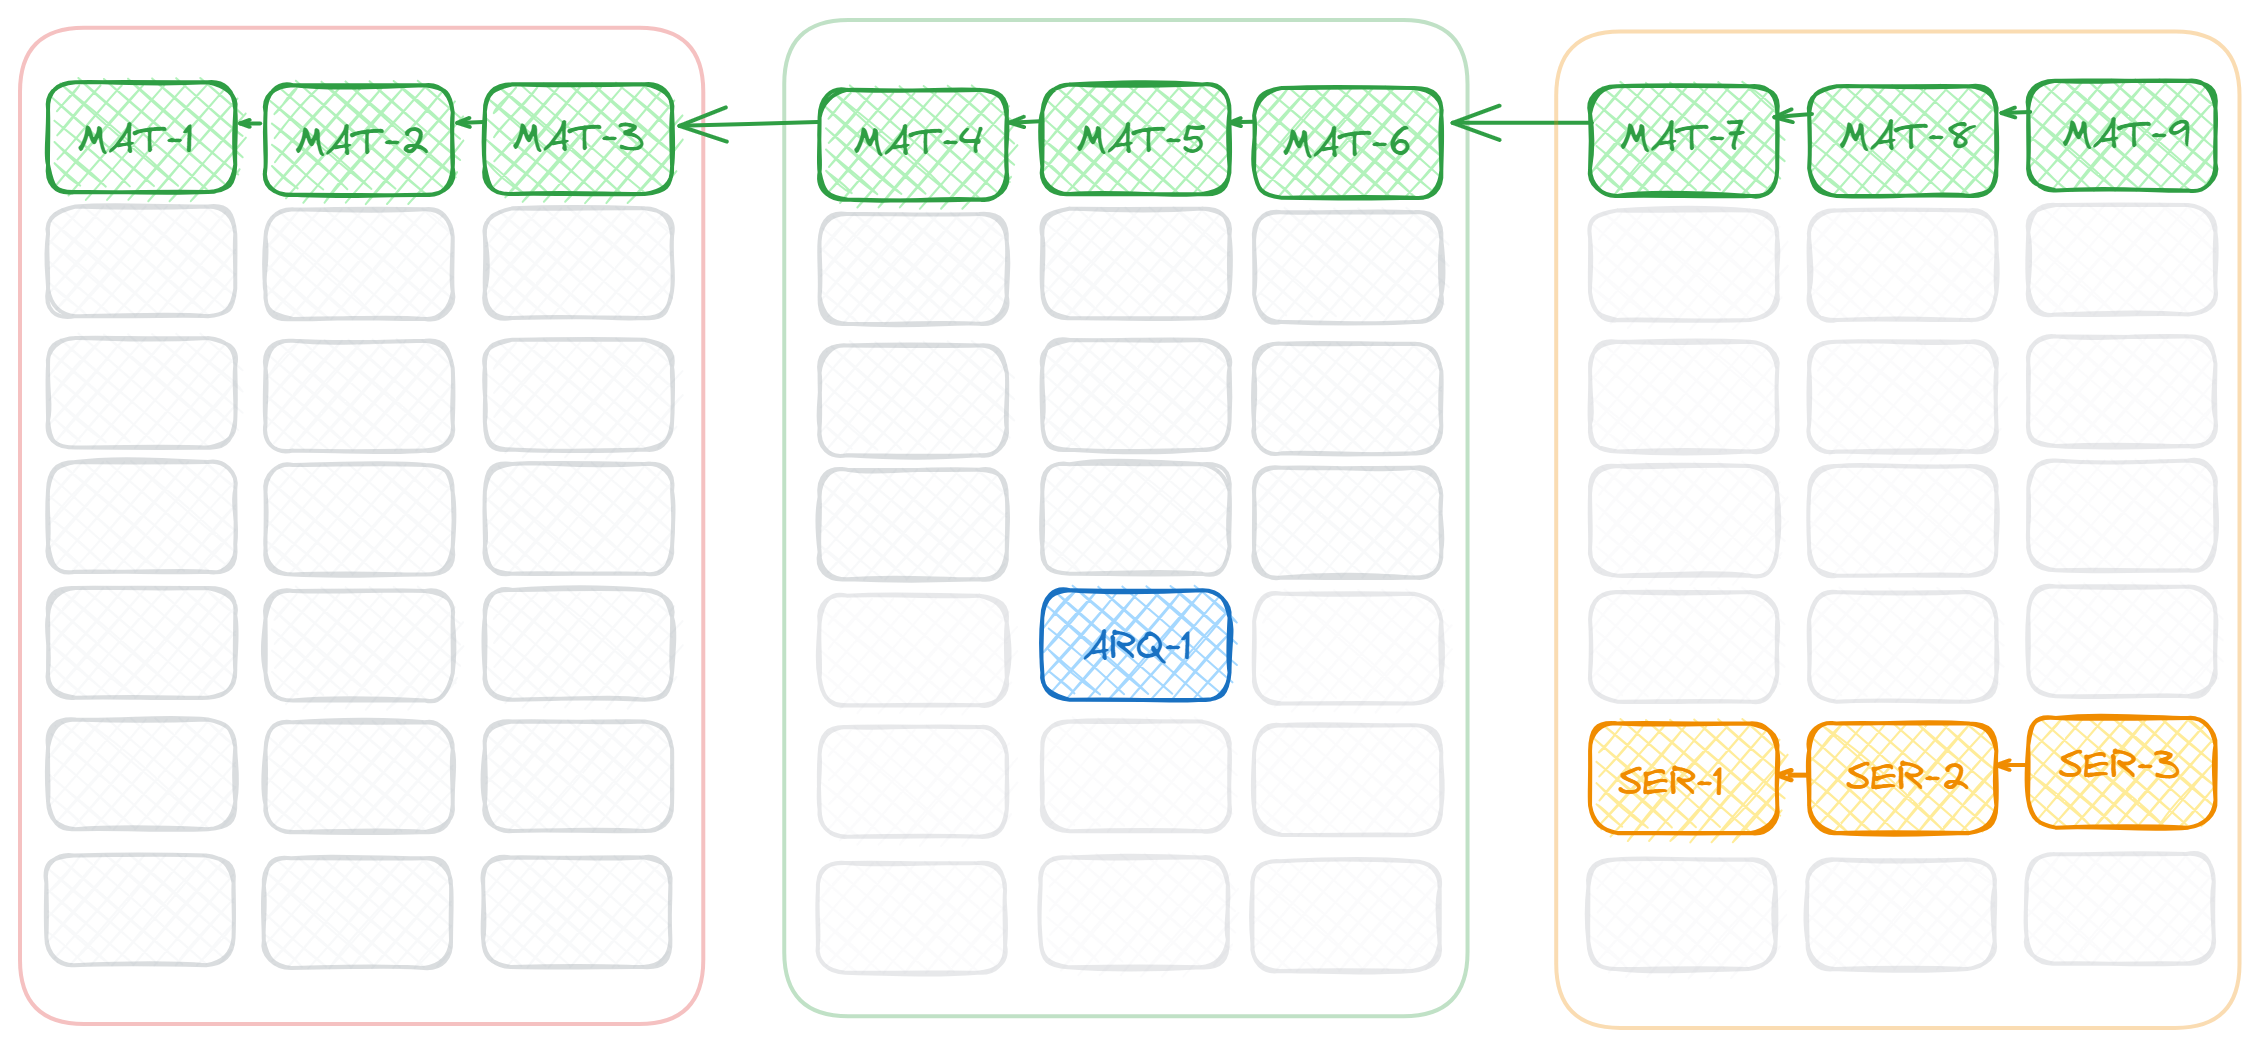
\includegraphics[width=\textwidth]{images/AG-Simple-Serial-Squeme.png}
    \caption{Mapa curricular simplificado de ejemplo: Caso 1.}
    \label{fig:mapa_curricular_simplificado_caso_1}
\end{figure}

Teniendo un mapa curricular como el de la figura \ref{fig:mapa_curricular_simplificado_caso_1}, cada materia tiene una lista de asignaturas que dependen de ella. Por ejemplo: %\\
\begin{itemize}
    \item MAT-7 tiene una lista de materias dependientes donde se hallan MAT-8 y MAT-9.
    \item MAT-6 tiene una lista de materias dependientes donde se hallan MAT-7, MAT-8 y MAT-9.
\end{itemize}

Cuando una materia, por ejemplo ARQ-1, no tiene ninguna asignatura en su conjunto de materias dependientes, se le considera una materia débilmente seriada. Esto significa que ARQ-1 puede ser cursada sin tener ninguna otra materia como requisito previo. En otras palabras, no existen restricciones de seriación que limiten la capacidad de cursar ARQ-1 en función de otras asignaturas.

Ahora, si una materia es marcada como ``reprobada", todas las materias pertenecientes a la lista de materias dependientes de esa materia reprobada se marcarán como ``deshabilitadas". Este proceso se aplica recursivamente a todas las materias dependientes de las materias deshabilitadas. Es decir, si una materia directamente dependiente de la materia reprobada se deshabilita, entonces todas las materias que dependen de esa materia también se deshabilitarán. La materia originalmente marcada como reprobada, sin embargo, será apta para volver a cargarse en futuros intentos académicos.
    
De manera similar, si una materia es seleccionada por el usuario y se encuentra dentro de al menos un conjunto de materias marcadas como reprobadas o no cursadas, esta materia también será marcada como ``deshabilitada". Este proceso garantiza que no se incluyan materias que tengan dependencias no cumplidas o que hayan sido reprobadas previamente, garantizando así la coherencia del horario académico del estudiante.

Esta delimitación se puede representar mediante una serie de condiciones algebraicas que describen el proceso de manera precisa.

Se define \( M \) como una materia existente en el plan académico de la carrera, \( R \) como una materia marcada como reprobada o no cursada, \( P \) como el conjunto de materias con posibilidad de carga, y \( N \) como el conjunto de materias sin posibilidad de carga.

Entonces, estas condiciones pueden expresarse de la siguiente manera:

\begin{itemize}
    \item Si \( M \) no pertenece al conjunto de dependientes de \( R \) y no está en el conjunto \( N \), entonces \( M \) pertenece al conjunto \( P \).
    \item Si \( M \) pertenece al conjunto de dependientes de \( R \), entonces \( M \) se coloca en el conjunto \( N \) y se elimina de \( P \).
\end{itemize}

Esto se puede expresar en términos algebraicos de la siguiente manera:

\begin{equation}
    \begin{split}
        (M \notin R[\text{dependientes}]) \wedge (M \notin N) \implies M \in P \\
        M \in R[\text{dependientes}] \implies (M \in N) \wedge (M \notin P )
    \end{split}
    \label{eq:condicion_de_seriacion_para_filtro_de_materias.}
\end{equation} \myequations{Condición de seriación para filtro de materias.}

Esta expresión algebraica define de manera clara y precisa las condiciones bajo las cuales una materia puede ser considerada para su carga en función del estado de otras materias y sus dependencias.

\begin{figure}[h]
    \centering
    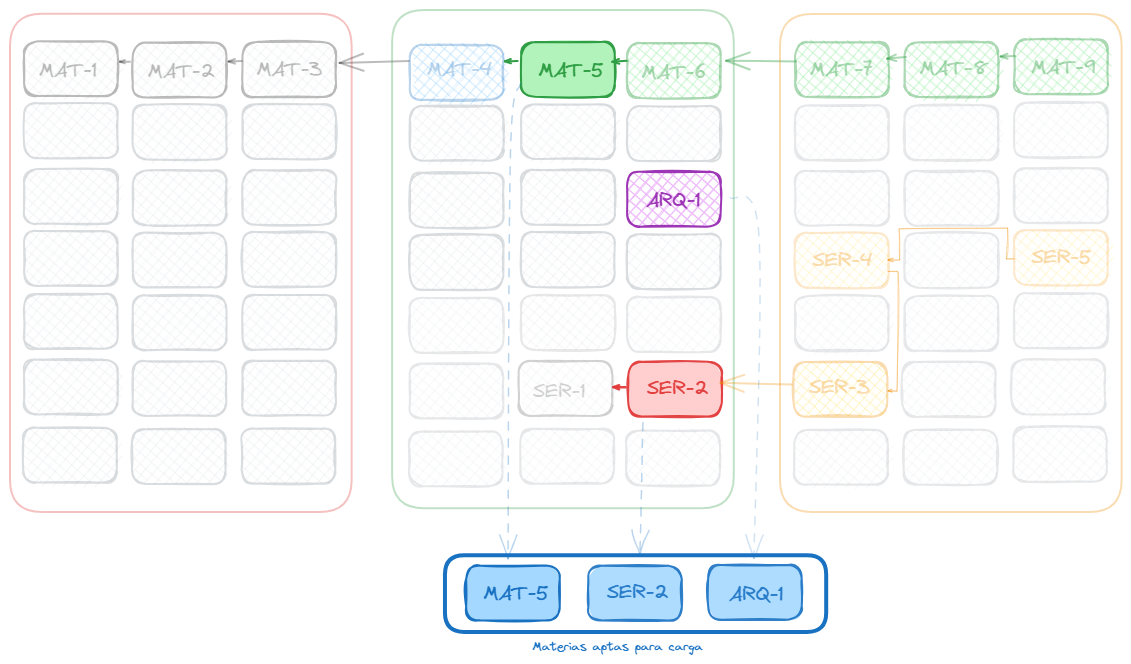
\includegraphics[width=0.8\textwidth]{images/AG-Simple-Serial-Squeme-3.png}
    \caption{Mapa curricular simplificado de ejemplo: Caso 2.}
    \label{fig:mapa_curricular_simplificado_caso_2}
\end{figure}

Para ilustrar este proceso, supongamos que el usuario ha aprobado las asignaturas MAT-4, pero ha reprobado SER-2 y no ha cursado ARQ-1. En este caso, las únicas materias disponibles para ser cargadas serán MAT-5, ya que es la continuación de MAT-4, SER-2, que es la materia que podrá volver a cursar en un nuevo intento académico, como se muestra en el mapa curricular simplificado de ejemplo en la figura \ref{fig:mapa_curricular_simplificado_caso_2}, y ARQ-1, que fue marcado como no cargada, y podrá ser cursada en el curso entrante como primera oportunidad.


Estas materias son recopiladas dentro de un nuevo conjunto, que en el diagrama es ilustrado como ``Materias aptas para carga", por otro lado, la materia SER-5, aunque no sea directamente dependiente de SER-2, está dentro de la línea de seriación gracias de SER-4 que depende de SER-3 que a su vez depende de SER-2, lo que significa que todas esas materias listadas deberán ser deshabilitadas, de esta manera solo las asignaturas que tienen su lista dependietes aprobadas, pueden pasar a la siguiente etapa.

\subsubsection{Filtrado de materias por disponibilidad horaria} \label{filtrado_de_materias_por_disponibilidad_horaria}

Una vez que hemos definido las materias del alumno, seleccionando solo aquellas que se ajustan a su estado académico actual, es necesario realizar un filtrado adicional basado en la disponibilidad de las materias para el próximo curso. Este paso es fundamental para garantizar la eficacia del algoritmo. En cada cuatrimestre, se establecen grupos de acuerdo con el número de alumnos y la disponibilidad de maestros en la carrera. Para los propósitos prácticos de nuestro algoritmo, nos basamos en los grupos abiertos durante el periodo de Enero-Abril de 2024. Dado que los números de grupo varían según el curso, esto influye directamente en la disponibilidad de las materias para su carga. Por lo tanto, debemos realizar un filtro adicional en nuestra lista de materias aptas para cargar, eliminando aquellas que no estén disponibles en el curso entrante, específicamente, durante el periodo de Enero-Abril de 2024.

Esta información se comunica a los alumnos a través de una lista que contiene los calendarios de todos los grupos disponibles. Cada horario \( S \) contiene las materias \( M \) ubicadas en su franja horaria correspondiente para cada grupo. Para facilitar la gestión de datos, nuestro equipo ha convertido este archivo a un formato de serialización de datos, lo que permite un acceso más accesible para el equipo de desarrollo sin agregar complejidad a la lectura de los datos. Estos horarios se presentan como un conjunto \( C \), que engloba todos los horarios \( S \) disponibles para el próximo periodo.


Cada horario \( S \) pertenece a un grupo \( S_{\text{grupo}} \), que según la cantidad de alumnos, pueden ser enumerados alfabéticamente de la A a la Z y a un cuatrimestre \( S_{\text{cuatrimestre}} \) en específico. Los horarios contienen una lista de asignaturas \( M \) que corresponden a las materias pertenecientes a ese cuatrimestre según el mapa curricular de la carrera (ver Figura \ref{fig:mapa_curricular_ids_2017}). Cada materia perteneciente al horario \( S \) contiene atributos como \( M_{\text{id}} \), que es un identificador único para identificar una asignatura entre todas las disponibles en el periodo; \( M_{\text{nombre}} \), que corresponde al nombre común de la materia; \( M_{\text{canonical}} \), que corresponde al identificador único de la materia sin procesar a la que hace referencia, definida en la sección \ref{eq:arreglo_materias_sin_procesar}; \( M_{\text{maestro}} \), que hace referencia al nombre del docente que imparte la materia para el grupo y cuatrimestre en específico; y \( M_{\text{[horas]}} \), a un arreglo de horas que representa a qué franja horaria de la semana ocupa dicha asignatura. Cada hora está representada siguiendo la definición de la sección \ref{franjas-horarias}.


En este sentido, podemos sintetizar cada parte de esta lista de la siguiente manera:

% Aqui no
\begin{gather*} 
    C: ([S]) \\
    S_i: (\text{cuatrimestre}_i, \text{grupo}_i, \text{[M]}_i) \\
    M_{ik}: (\text{id}_{ik}, \text{nombre}_{ik}, \text{canonical}_{ik}, \text{maestro}_{ik}, \text{[horas]}_{ik}) \\
    \label{eq:definicion_lista_de_horarios_por_periodo}
\end{gather*} 
\myequations{Lista de horarios disponible por periodo y sus atributos}
\clearpage
\begin{figure}[h]
    \centering
    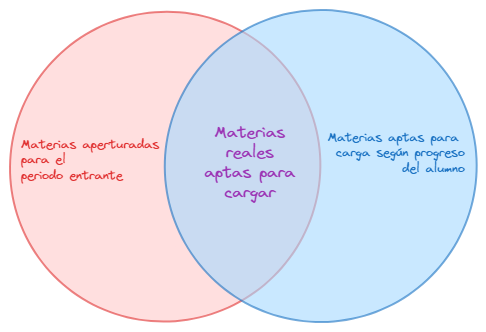
\includegraphics[width=0.4\textwidth]{images/Real-Assignatures-to-Load.png}
    \caption{Diagrama de materiales reales de carga.}
    \label{fig:materias_reales_de_carga}
\end{figure}

Ahora, para obtener las materias reales para carga, debemos de tomar aquellas asignaturas disponibles de carga, que cumplen con la regla definida en la ecuación \ref{eq:condicion_de_seriacion_para_filtro_de_materias.}, y conservar únicamente aquellas materias que también estén presente dentro de las asignaturas de los horarios que están en la lista de grupos disponibles para el periodo próximo, como se representa en la figura \ref{fig:materias_reales_de_carga}.

La definición de la existencia de una materia \( M \) en el conjunto de materias reales de carga \( R \) se expresa como:

\begin{equation}
    M \in R \iff M \in S, \text{ para algún } S \in G
    \label{eq:definicion_materiales_reales_de_carga}
\end{equation} 
\myequations{Definición de materiales reales de carga.}

Donde:
\begin{align*}
    & M \text{ es una materia.} \\
    & R \text{ es el conjunto de materiales reales de carga.} \\
    & S \text{ es una asignatura.} \\
    & G \text{ es el conjunto de horarios disponibles en la lista de horarios disponibles \( L \).}
\end{align*}

\subsection{Cuantificación de los datos} \label{cuantifiacion_de_datos}

Otra parte importante del proceso previo al procesamiento de las materias por el algoritmo genético, es la cuantificación de los datos, es decir, añadir valores numéricos a las materias con el fin de realizar operaciones algebraicas y definir de una manera más concreta si una materia es apta para el alumno.

Después de realizar las delimitaciones de las materias, como se detalló en las secciones \ref{depuracion_de_materias} y \ref{filtrado_de_materias_por_disponibilidad_horaria}, nos queda una lista de materias que son aptas para ser procesadas por el algoritmo genético. Sin embargo, es necesario agregar información adicional y eliminar información innecesaria para mejorar la eficiencia del programa y garantizar que los datos proporcionados al algoritmo genético sean óptimos para generar un horario ideal.

En este sentido, se eliminarán ciertas propiedades de las materias disponibles de carga, como ``dependientes", ``dependencias" y ``status", que fueron utilizadas únicamente en la sección \ref{depuracion_de_materias} para eliminar las materias con seriaciones incompletas.

Por otro lado, se introducen nuevas propiedades de la materia. Sin embargo, para los fines explicativos de este documento, nos centraremos únicamente en dos atributos principales: el Umbral de Relevancia (\( \mu \)), también conocido internamente como peso, y un horarios \( H \) que describen que franja horaria de la semana se lleva acabo la clase de la materia en cuestión. La definición de estas horas se especifican en la sección \ref{franjas-horarias}.

\begin{equation}
    M: (\mu, [H])
    \label{definicion_de_materia_apta_para_procesamiento.}
\end{equation} \myequations{Definición simplificada de materia apta para procesamiento.}

Estas materias pertenecen a un conjunto de materiales reales de carga $D$ que se adjunta a otro conjunto de entrada $E$ que se enviará al servidor del algoritmo genético para su procesamiento. Este conjunto $E$ posee propiedades adicionales que hacen referencia a información adicional para el funcionamiento, como cuatrimestre actual del alumno y configuraciones técnicas para el algoritmo gnético.

Descrito explícitamente podríamos decir

\begin{gather*}
        D: \{ M_1, M_2, \dots, M_i \} \\
        E: (D, C)
    \label{definiciones_de_datos_de_entrada.}
\end{gather*} \myequations{Definiciones de datos de entrada.}

Este conjunto de datos son los que serán procresado por el algoritmo genético para generar el horario más óptimo para el alumno, abordemos cada uno de los campos a continuación.

\subsubsection{Umbral de relevancia}
\label{umbral_relevancia}
El umbral de relevancia, también conocido como peso, es un número entero mayor a 0 asociado a cada materia. Este número indica la importancia de la materia y es utilizado por la función que determina el horario final del alumno.

El cálculo del umbral se rige por las siguientes reglas:

\begin{itemize}
    \item Por cada materia dependiente, se añade 1 punto al umbral.
    \item Si la materia se encuentra en un cuatrimestre menor al cuatrimestre actual del alumno, se suma 1 punto al umbral por cada cuatrimestre de diferencia entre el último cuatrimestre actual y el cuatrimestre de la materia.
\end{itemize}

Para un mejor entendimiento, dividiremos el cálculo de este umbral en dos partes: calcular el peso de las dependientes y el cálculo de peso por distancia de cuatrimestre.

Para calcular el umbral de relevancia por dependientes, primero definimos el conjunto de materias dependientes como \( D \), donde \( |D| \) representa el número de materias dependientes de una materia. Entonces, el umbral de relevancia \( \mu_r \) por dependientes se calcula como:

\begin{equation}
    \mu_r = |D| + \sum_{d \in D} \mu_r
    \label{eq:umbral_relevancia_por_dependientes}
\end{equation} 
\myequations{Cálculo de umbral de relevancia por dependientes.}

Donde:
\begin{align*}
    & \mu_r \text{ es el umbral de relevancia por dependientes.} \\
    & D \text{ es el conjunto de materias dependientes de una materia.} \\
    & |D| \text{ es el número de materias dependientes de una materia.} \\
    & \mu_r \text{ es el umbral de relevancia de cada materia dependiente.}
\end{align*}

Para la primera parte, que es el cálculo de peso por dependientes, el conjunto de materias se recorre de forma inversa, es decir, de mayor cuatrimestre a menor cuatrimestre. Por cada materia en dependientes, se suma 1 punto a su peso; por cada materia dependiente, se suma el peso de esa materia. Esto se representa visualmente en la Figura \ref{fig:ejemplo_ilustrativo_calculo_de_relevancia_por_dependiente}.

\begin{figure}[h]
    \centering
    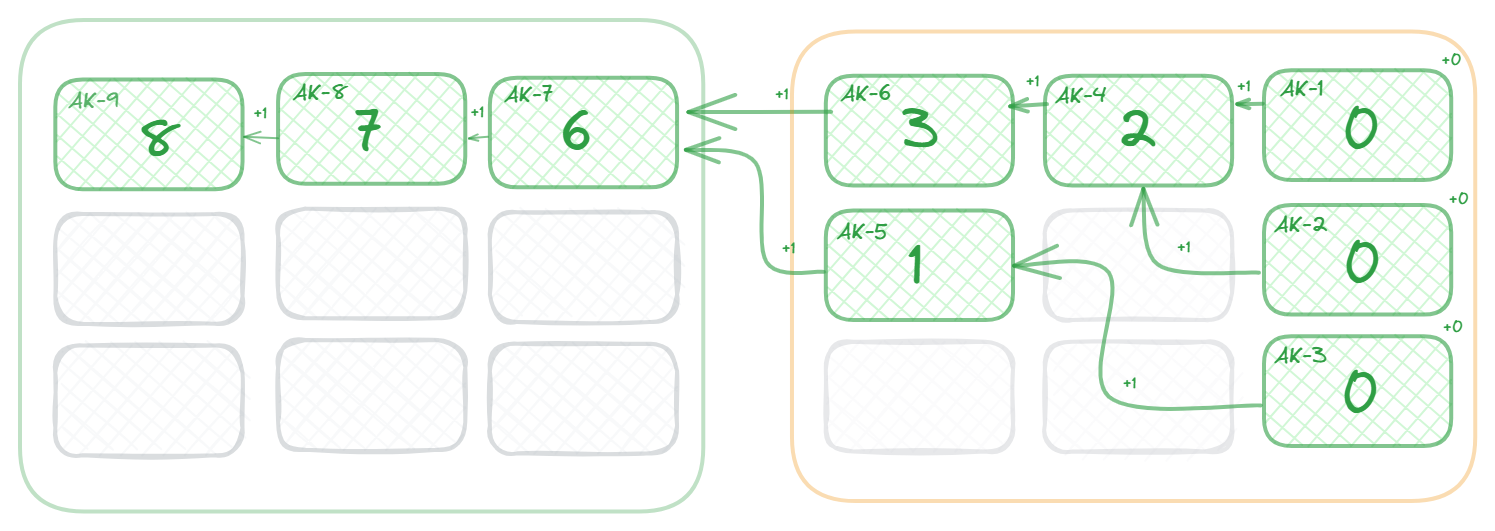
\includegraphics[width=0.6\textwidth]{images/relevance-by-dependents.png}
    \caption{Ejemplo ilustrativo de cálculo de relevancia por dependiente.}
    \label{fig:ejemplo_ilustrativo_calculo_de_relevancia_por_dependiente}
\end{figure}

En la ilustración \ref{fig:ejemplo_ilustrativo_calculo_de_relevancia_por_dependiente}, se muestra el proceso de cálculo de las materias. El peso de las materias de AK-1 al AK-3 es 0, ya que al ser la última materia del plan curricular, no tiene materias que dependan de ella.

Podemos ver que la materia AK-4 tien un peso de 2. Esto resulta de tener dos materias que dependen de ella: AK-1 y AK-2, sumando 1 punto por cada una. Además, se suma el valor de dichas dependientes, que son 0. Al final, el peso de la materia mostrada será de 2.

Tomemos un ejemplo más complejo, como el de la materia AK-7, que tiene dos materias dependientes: AK-6 y AK-5. Ambas suman 1 punto al peso de AK-7, teniendo un peso inicial de 2. Ahora debemos sumar el peso de cada dependiente a la materia AK-7, que para AK-6 sería 3 y para AK-5 sería 1. Teniendo estos valores, tendríamos que el valor total del peso de AK-7 es 6, ya que $3+1+1+1 = 6$.

De esta forma, nos aseguramos de que las materias con la mayor cantidad de dependientes tengan prioridad al generar el horario, en comparación con las materias con pocas dependientes.

Es importante realizar este cálculo antes que todo, de esta forma evitamos tomar en cuenta pesos que no corresponden exclusivamente a la cantidad de materias dependientes de cada asignatura.

El umbral de relevancia por distancia se calcula como la diferencia entre el cuatrimestre de la materia ($M$) y el cuatrimestre del alumno ($C$), siempre y cuando $M$ sea mayor que $C$. De lo contrario, no se suma nada y el umbral es igual a $0$.

\begin{equation}
    \mu_d = \begin{cases} M - C, & \text{si } M > C \\ 0, & \text{si } M \leq C \end{cases}
    \label{eq:umbral_distancia}
\end{equation}
\myequations{Cálculo de umbral de relevancia por distancia.}

Donde:
\begin{align*}
    M & : \text{Cuatrimestre de la materia.} \\
    C & : \text{Cuatrimestre del alumno.} \\
    \mu_d & : \text{Umbral de relevancia por distancia.}
\end{align*}

Para el cálculo de relevancia por distancia, usamos una operación un poco más simple. Sabiendo el cuatrimestre del alumno, a cada materia de cuatrimestre menor al cuatrimestre del alumno, se le va a sumar un punto por cada materia de distancia que tenga al cuatrimestre actual del usuario.

\begin{figure}[h]
    \centering
    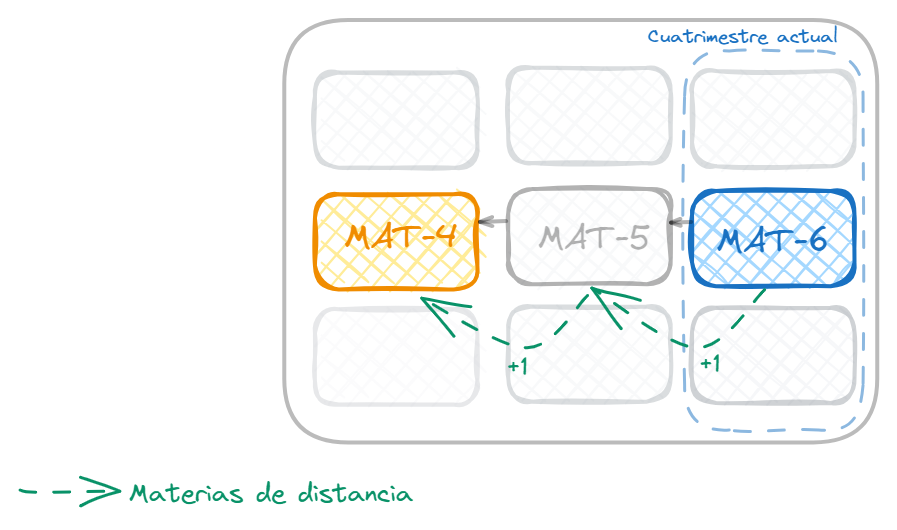
\includegraphics[width=0.6\textwidth]{images/AG-Simple-Serial-Umbral-Relevancia.png}
    \caption{Ejemplo ilustrativo de cálculo de relevancia por distancia.}
    \label{fig:ejemplo_ilustrativo_calculo_de_relevancia_por_distancia}
\end{figure}

Por ejemplo, consideremos el caso del umbral de la materia MAT-4 de la Figura \ref{fig:ejemplo_ilustrativo_calculo_de_relevancia_por_distancia} para un alumno en sexto semestre, mientras que el cuatrimestre donde se halla la materia MAT-4 está a 2 cuatrimestres de distancia. Por cada cuatrimestre de diferencia entre el cuatrimestre actual del alumno y el cuatrimestre de la materia, se suma un punto adicional al umbral de relevancia de la materia. Por lo tanto, se añadirán 2 puntos al umbral de MAT-4.

Adicionalmente, después de todos los cálculos realizados, se sumará 1 punto adicional a cada umbral para evitar tener materias con 0 puntos y mejorar la eficiencia del cálculo de nuestro algoritmo genético.

Finalmente, nuestro umbral de relavancia es el resultado de la suma de estos dos umbrales más 1, como se muesta a continuación.

\begin{equation}
    \mu = \mu_r + \mu_d + 1
    \label{eq:umbral_relevancia}
\end{equation}
\myequations{Umbral de relevancia.}
\clearpage
\subsubsection{Franja horaria}\label{franjas-horarias}
La franja horaria es una forma numérica de definir que horas de la semana se imparte una clase, esto se puede definir a través de números enteros entre el 1 y el 45, cada número representa una hora entre las 8:00hrs. a las 17:00hrs. de algún día entre lunes a viernes como se muestra en la ilustración \ref{fig:franja-horaria}.

\begin{figure}[h]
    \centering
    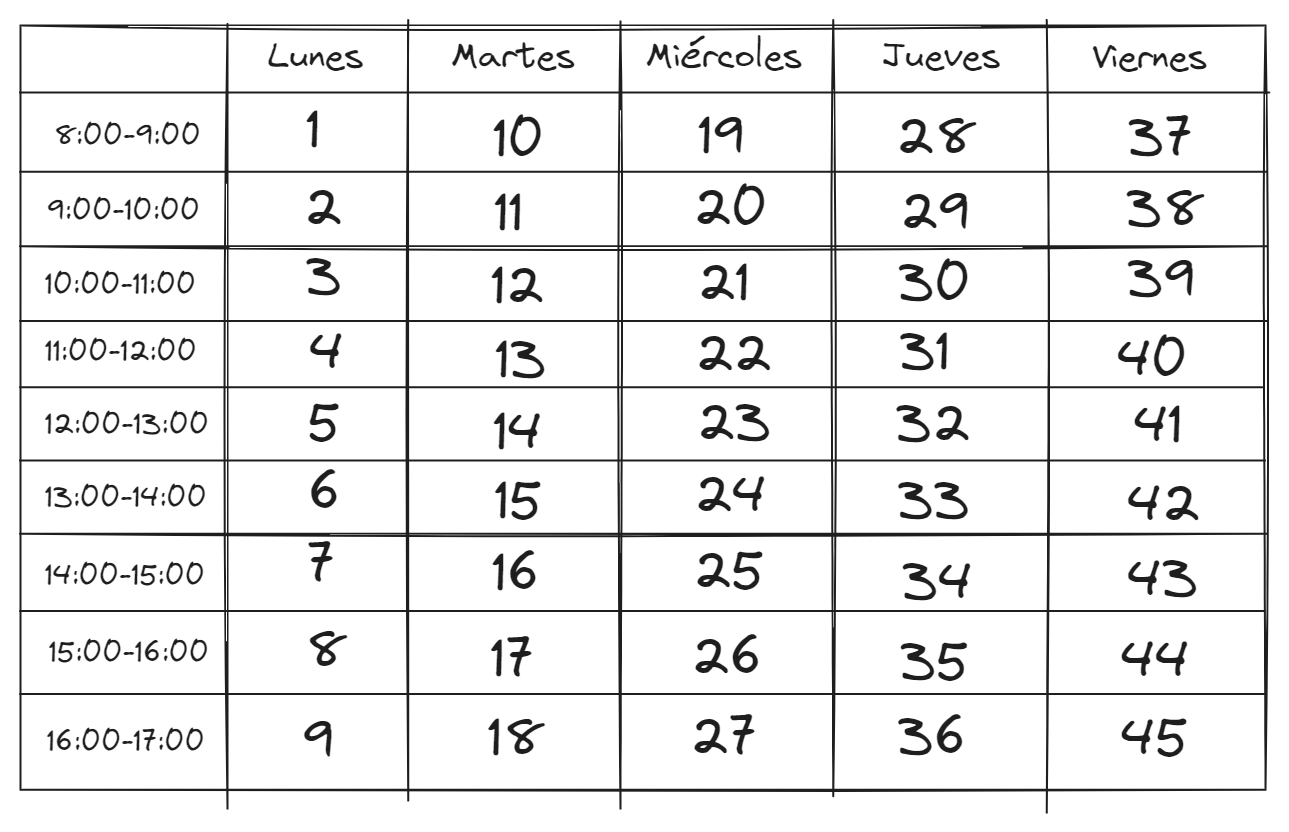
\includegraphics[width=0.5\textwidth]{images/franja-horaria.png}
    \caption{Representación de los valores de la franja horaria.}
    \label{fig:franja-horaria}
\end{figure}

De esta forma, una materia que tenga un franja horaria con los siguientes datos 
$[2, 3, 10, 26, 27, 38, 39, 40]$ tendría una distribución visual en el horario como se muestra en la figura \ref{fig:franja-horaria-caso}

\begin{figure}[h]
    \centering
    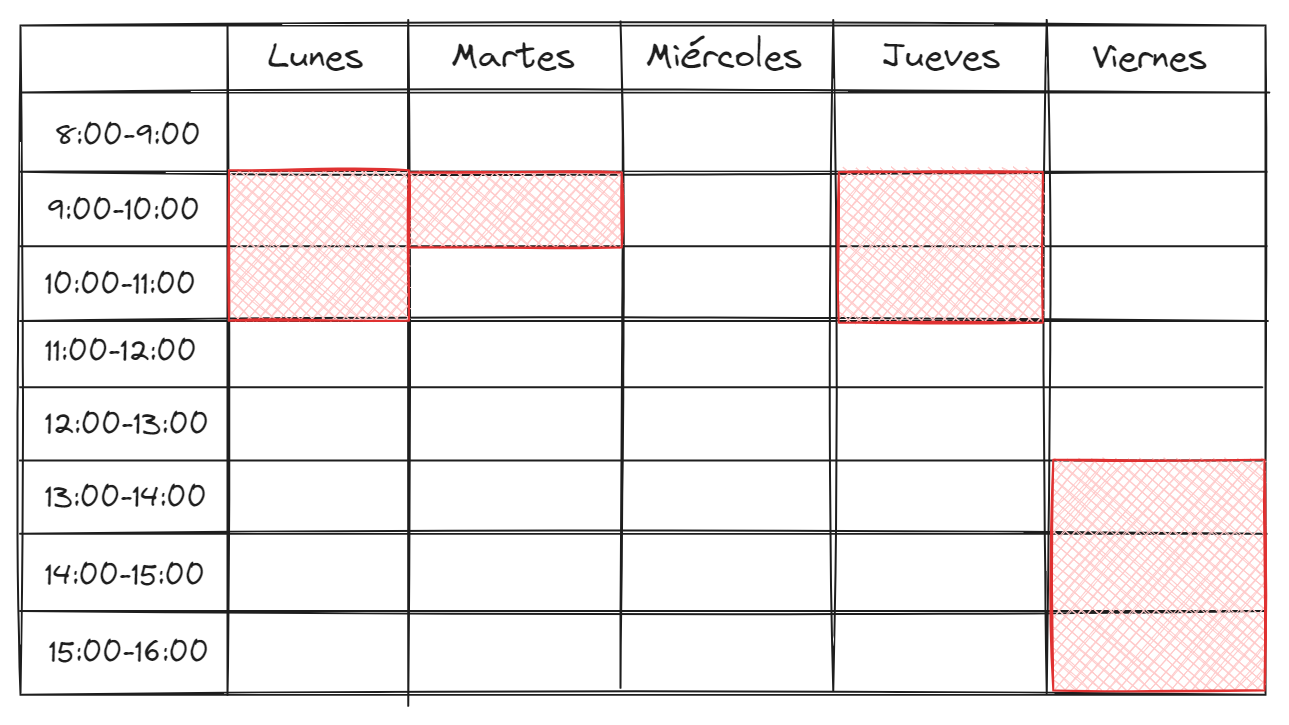
\includegraphics[width=0.5\textwidth]{images/franja-horaria-caso.png}
    \caption{Franja horaria: Ejemplo 1.}
    \label{fig:franja-horaria-caso}
\end{figure}

\subsection{Procesamientode la información} \label{procesamiento_de_la_informacion}
Ahora, hablaremos sobre cómo nuestro algoritmo procesó a las materias reales para carga (ver definición \ref{eq:definicion_materiales_reales_de_carga}), para esto es indispensables definir 3 nuevos concepto que nos ayudó a tener un registro de aquellos horarios que cumplen con todos los criterios para poder ser cursado, y evaluar la mejor alternativa, estos conceptos son: semilla, longitud de semilla y base aritmética, que se explica a profundidad en las secciones \ref{semilla}, \ref{longitud_de_semilla} y \ref{base_aritmetica} respectivamente.

\subsubsection{Semilla} \label{semilla}
La semilla corresponde a un identificador único para cada nuevo horario o individuo generado, consta de una longitud de carácteres definido en la longitud de semilla de la sección \ref{longitud_de_semilla}, y sirve para poder replicar un individuo en cualquier parte del tiempo y bajo el mismo contexto de materias. Esto permite replicar de forma seguro e inequívoca a aquellos horarios pertinentes para visualización.

\subsubsection{Longitud de semilla}\label{longitud_de_semilla}
La longitud de semilla correponde a la cantidad de carácteres que tendrá una semilla, esto es importante para hacer que las semillas generadas cubran por completo todas las posibles combinaciones de horarios y evitando dejar generaciones imposibles de replicar o semillas tan largas que abarcan generaciones fuera del rango de posibilidades. 

Este número se genera tomando en cuenta la cantidad de materias reales de carga (ver visualización \ref{fig:materias_reales_de_carga}), es decir, si en una instancia del algoritmo genético hay 7 materias reales de carga, la longitud de los carácteres de la semilla será de 7. El valor de los carácteres varían según lo definido en la sección \ref{base_aritmetica}.

\subsubsection{Base Aritmética} \label{base_aritmetica}
La base aritmética representa el rango de incremento de cada carácter en la semilla, es decir, una base aritmética de 2, también conocido como binario, los valores en el cual el carácter puede incrementar son dos posibilidades: 0 y 1.

Este valor se define tomando el valor máximo de grupos abiertos para una materias reales disponibles existente en la lista de materiales reales de carga que se envía a través de los datos de entrada definido en la ecuación \ref{definiciones_de_datos_de_entrada.}.

Para ilustrar estos conceptos de una forma más clara, tomemos la ilustración \ref{fig:semilla-base-aritmetica} de ejemplo.

\begin{figure}[h]
    \centering
    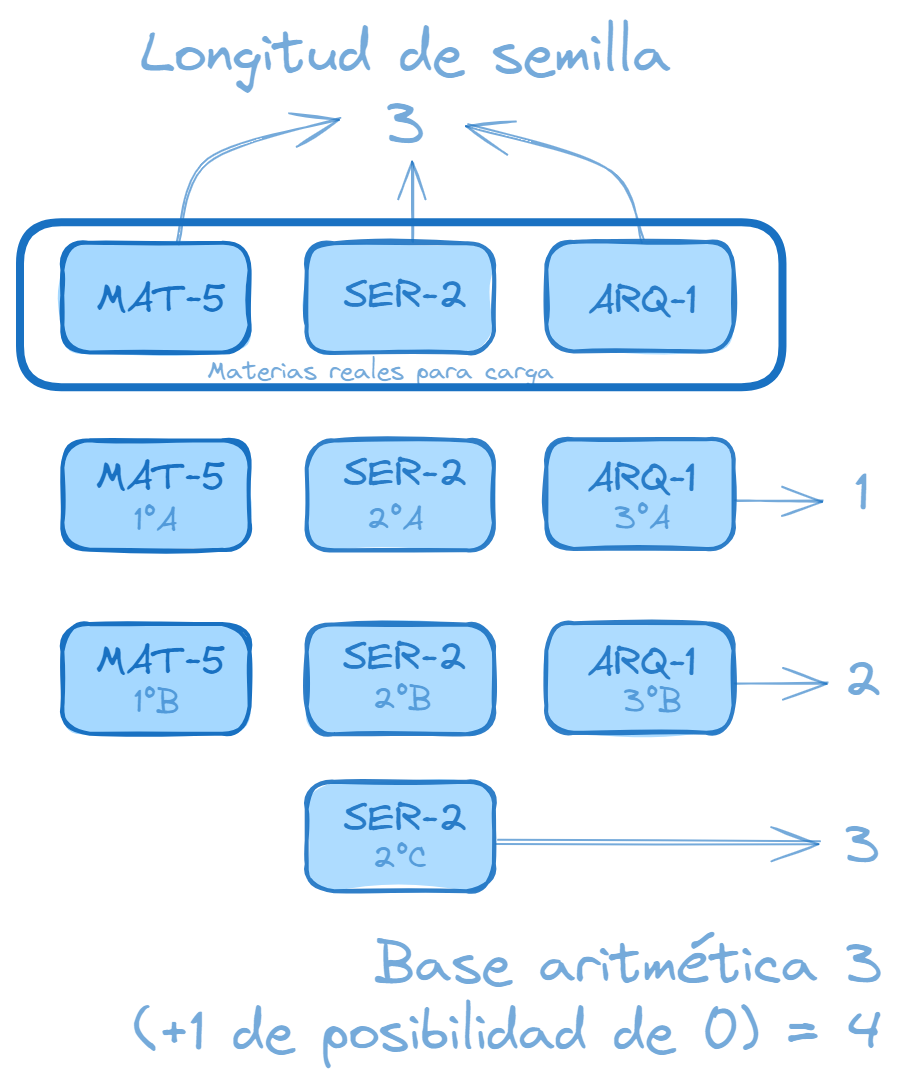
\includegraphics[width=0.4\textwidth]{images/semilla.png}
    \caption{Visualización de longitud de semilla y base aritmética.}
    \label{fig:semilla-base-aritmetica}
\end{figure}

En la ilustración anterior \ref{fig:semilla-base-aritmetica} podemos ver como para ese caso, la base aritmética es 4, y la longitud de semilla es 3.

La longitud, como se define en la sección \ref{longitud_de_semilla}, es el valor de las materias reales para carga de esa instancia del algoritmo genético, que en este caso son: MAT-5, SER-2 y ARQ-1, dando como resultado una longitud de semilla de 3.

Para la base aritmética, se considera la mayor cantidad de grupos disponibles (ver \ref{filtrado_de_materias_por_disponibilidad_horaria}) para alguna materia existente en la lista de materias reales de carga en la instancia del algoritmo genético actual. Para el ejemplo anterior, esto es 3, debido a que SER-2 tiene tres grupos disponibles para cursar dicha materia, que son: 2°A, 2°B y 2°C. A esta longitud, debemos incrementar una base más, para que pueda interpretarse el 0 como un dígito válido para la semilla y tener una buena interpretación de la semilla como se define en la sección \ref{decodificacion_se_semilla}.

\subsubsection{Decodificación de semilla}\label{decodificacion_se_semilla}
La decodificación de semilla es la parte del algoritmo en la que dada una semilla, y ya defininido su longitud y base aritmética, procedemos a decodificar a qué materias hace referencia dicha semilla, para ilustrar este paso tomemos la figura \ref{fig:visualización_de_decodificación_de_semilla}.

\begin{figure}[h]
    \centering
    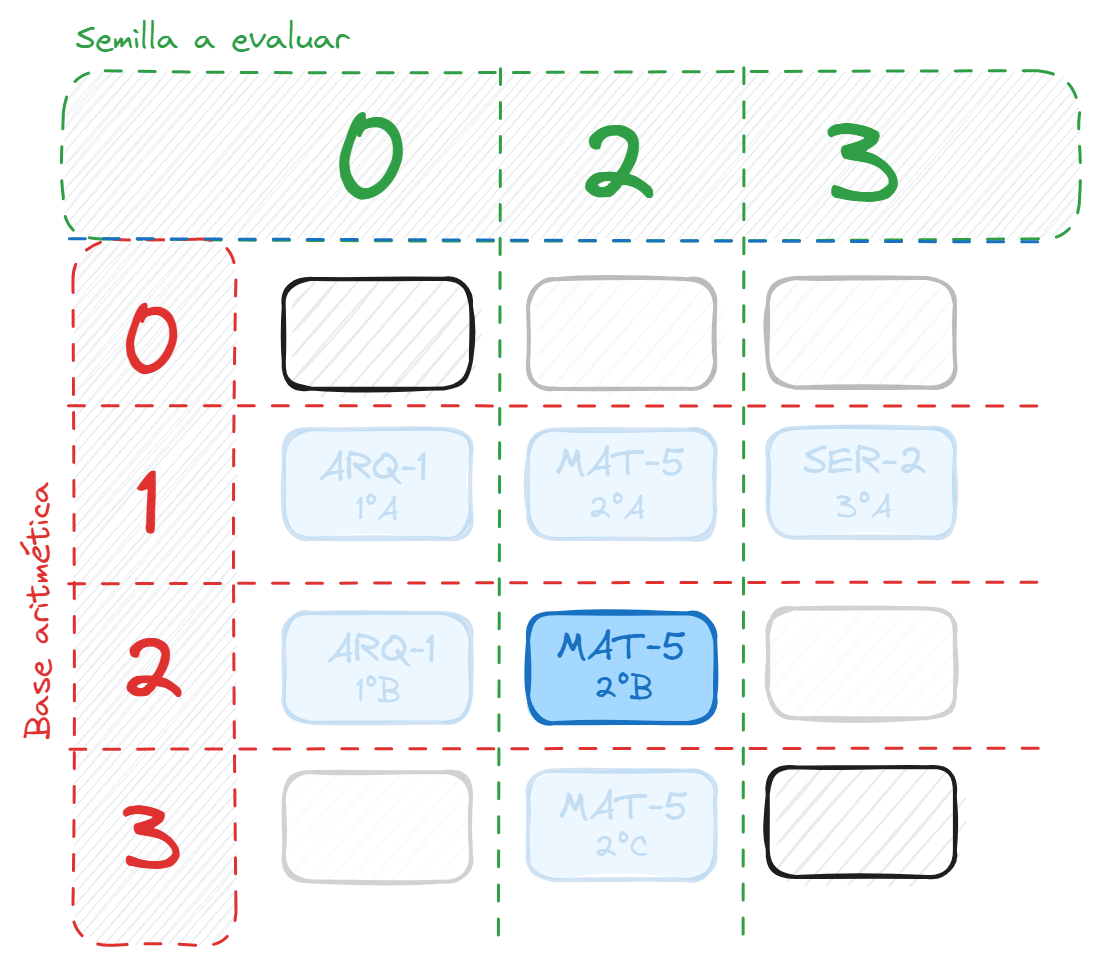
\includegraphics[width=0.5\textwidth]{images/seed-calc.png}
    \caption{Visualización de decodificación de semilla.}
    \label{fig:visualización_de_decodificación_de_semilla}
\end{figure}

En el ejemplo anterior, la semilla tiene una longitud de 3, y ina base aritmética de 4, esto lo calculamos previamente como lo explicamos en las secciones \ref{longitud_de_semilla} y \ref{base_aritmetica}, lo que nos indica que las semillas posibles oscilan entre "000" y "333".

El siguiente paso es ordenar las materias por su id canonical (ver sección \ref{filtrado_de_materias_por_disponibilidad_horaria}) de forma alfabética, este id, al ser único entre todas las materias, y al ordernarlo alfabeticamente nos permite tener una mayor consistencia al momento de codificar las semillas bajo el mismo contexto de materias.

Posteriormente, asignamos cada carácter de la semilla a una materia, y el valor corresponde a la alternativa o grupo de la materia en cuestión, estas materias seleccionadas se almacenan dentro de una lista llamada\textbf{lista de materias activas}, que es usada para saber si el individuo está con colisión o no (ver sección\ref{individuos}).

Si el valor del carácter es 0, la materia no se añade a la lista de materias activas, como es el caso de la materia ARQ-1 del ejemplo de la figura \ref{fig:visualización_de_decodificación_de_semilla}, por otro lado si el valor excede a la cantidad de posibilidades reales de la materia, esta materia tampoco es añadida a la lista de materias activas, como es el caso de la materia SER-2 del ejemplo de la figura \ref{fig:visualización_de_decodificación_de_semilla}.


\subsubsection{Individuos} \label{individuos}

Dentro del algoritmo genético implementado en la aplicación, conocemos como individuo a aquel objeto capaz de interpretar una semilla (ver sección \ref{semilla}), dado un contexto específico, es decir, una lista de materias reales de carga.

Con dicha interpretación de la semilla, puede calcular sus pesos totales y definirse como un individuo con colisiones o sin colisiones según los siguientes parámetros.

Un individuo es considerado \textbf{sin colisión} si, según la decodificación de la semilla (ver sección \ref{decodificacion_se_semilla}), ninguna hora de la franja horaria de cualquier materia perteneciente a la lista de materias activas se encuentra dentro de otra franja horaria de otra materia de la misma lista de materias activas. Matemáticamente, esto se expresa como:

\begin{equation}
    \text{sin\_colisiones}(i, j) = \begin{cases} 
        \text{verdadero}, & \text{si no hay colisión entre las franjas horarias de las materias } i \text{ y } j \\ 
        \text{falso}, & \text{en caso contrario}
    \end{cases}
    \label{eq:sin_colisiones}
\end{equation}
\myequations{Condición de individuo sin colisiones.}

donde $\text{no\_hay\_colisión}(i, j)$ es una función que retorna verdadero si no hay colisión entre las franjas horarias de las materias $i$ y $j$, y falso en caso contrario.

En caso contrario, se considera al individuo como \textbf{con colisiones}, y no es usado como posible horario apto para el alumno.

Independientemente del estado del individuo, se calcula un \textbf{peso total} para cada individuo calculado, que es la suma de todos los pesos de todas las materias existentes en la lista de materias activas. Matemáticamente, esto se expresa como:

\begin{equation}
    \text{peso\_total} = \sum_{i \in \text{materias\_activas}} \text{peso}(i)
    \label{eq:peso_total}
\end{equation}
\myequations{Cálculo del peso total de un individuo.}

donde $\text{peso}(i)$ es el peso de la materia $i$.

\section{Resultado y salida} \label{resultado_salida}

Tras finalizar todas las generaciones del algoritmo genético y evaluar a cada individuo generado en cada iteración, regresamos al usuario al usuario el horario del individuo sin colisión con mayor peso (o umbral de relevancia, ver seccion \ref{umbral_relevancia}). Para esto, decodificamos la semilla (ver sección \ref{individuos})del individuo con el umbral más alto y se lo enviamos al usuario para que la aplicación web renderice el horario correspondiente (ver figura \ref{fig:resultado}).


\section{Metodología} \label{metodologia}

En esta sección se presenta en detalle la metodología empleada para el desarrollo del algoritmo genético utilizado en la aplicación.

\subsection{Emparejamiento} \label{emparejamiento}

El proceso de emparejamiento es crucial en los algoritmos genéticos, ya que determina cómo se combinan los individuos para generar descendencia. En nuestro enfoque, utilizamos dos estrategias distintas para el emparejamiento: A2 y C2.

La estrategia A2 consiste en evaluar, para cada individuo de la población, si se cruzará con otro individuo basándose en un umbral de probabilidad de cruce ($P_c$). Si la evaluación es positiva, se selecciona aleatoriamente uno o más individuos como pareja para el cruce.

Por otro lado, la estrategia C2 implica el uso de múltiples puntos de cruza para el intercambio de información genética entre los individuos emparejados. Para cada pareja a cruzar, se elige aleatoriamente la cantidad de puntos de cruza, y luego para cada punto de cruza se selecciona aleatoriamente la posición en la secuencia genética (semilla) donde se realizará el intercambio.

La combinación de estas estrategias nos permite explorar de manera eficiente el espacio de búsqueda de soluciones al permitir una variedad de intercambios genéticos entre los individuos emparejados.

\subsection{Mutación} \label{mutacion}

La mutación es un operador esencial en los algoritmos genéticos, ya que introduce diversidad en la población y permite explorar nuevas soluciones. En nuestro enfoque, adoptamos la estrategia M2 para la mutación. Esta estrategia implica el intercambio de posición de caracteres de la semilla de un individuo (ver seccioón \ref{semilla}). En otras palabras, si un individuo sufre una mutación, se elige aleatoriamente una posición en su semilla y se intercambia el carácter en esa posición con otro carácter seleccionado aleatoriamente.

La estrategia M2 se seleccionó debido a su capacidad para modificar las soluciones existentes de manera no determinista, lo que puede ser beneficioso para explorar el espacio de búsqueda de manera más amplia.

\subsection{Poda} \label{poda}

La poda de la población es un paso importante para controlar el tamaño y la diversidad de la población en cada iteración del algoritmo genético, así como mejorar el rendimiento del algoritmo. En nuestro enfoque, implementamos la estrategia P2 para la poda. Esta estrategia implica una eliminación aleatoria de individuos de la población, asegurando que al menos el mejor individuo de la población se conserve en cada iteración. 

La elección de esta estrategia se basa en su capacidad para mantener una población diversa y promover la convergencia hacia soluciones óptimas al conservar los individuos más prometedores.


\section{Visualización y gráficos} \label{visualizacion_y_graficos}
En esta sección, a forma de galeria de imágenes, mostramos algunas de las interfaces implementadas para el aplicativo y algunas de las técnicas usada para hacer una experiencia de usuario agradable.

\subsection{Progreso actual} \label{progreso_actual}
Esta sección es donde el usuario selecciona que materias ha aprobado, reprobado y se ve visualmente qué materias son inhabilitadas por no cumplir su seriación, y cuales son las que pondrán ser cargadas.

\begin{figure}[h]
    \centering
    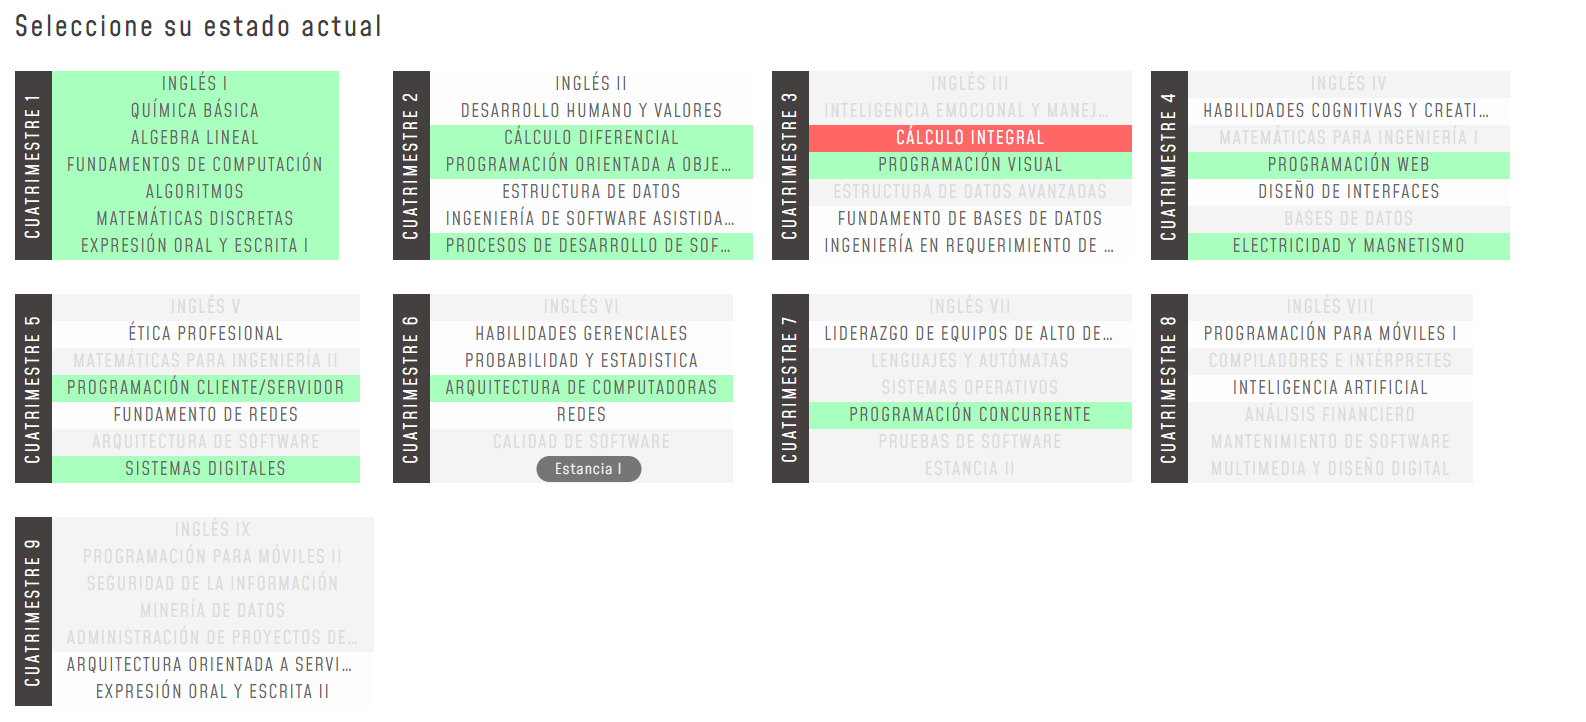
\includegraphics[width=0.7\textwidth]{images/current_status_real.png}
    \caption{Sección de selección de estado actual del usuario.}
    \label{fig:seccion_de_seleccion_de_estado_actual_del_usuario}
\end{figure}

A pesar de ser muy similar a la figura \ref{fig:captura_materias}, la figura \ref{fig:seccion_de_seleccion_de_estado_actual_del_usuario} es la vista que está implementada en la versión final del programa.

\subsection{Grupos disponibles} \label{grupos_disponibles}
Como vimos en la seccion \ref{filtrado_de_materias_por_disponibilidad_horaria}, la disponibilidad de una materia depende de los grupos que se aperturan en un periodo determinado, para mostrar estos grupos disponibles, nuestra aplicación tiene un apartado donde podemos ver aquellos grupos abiertos para el periodo que usa el algortimo genético.

\begin{figure}[h]
    \centering
    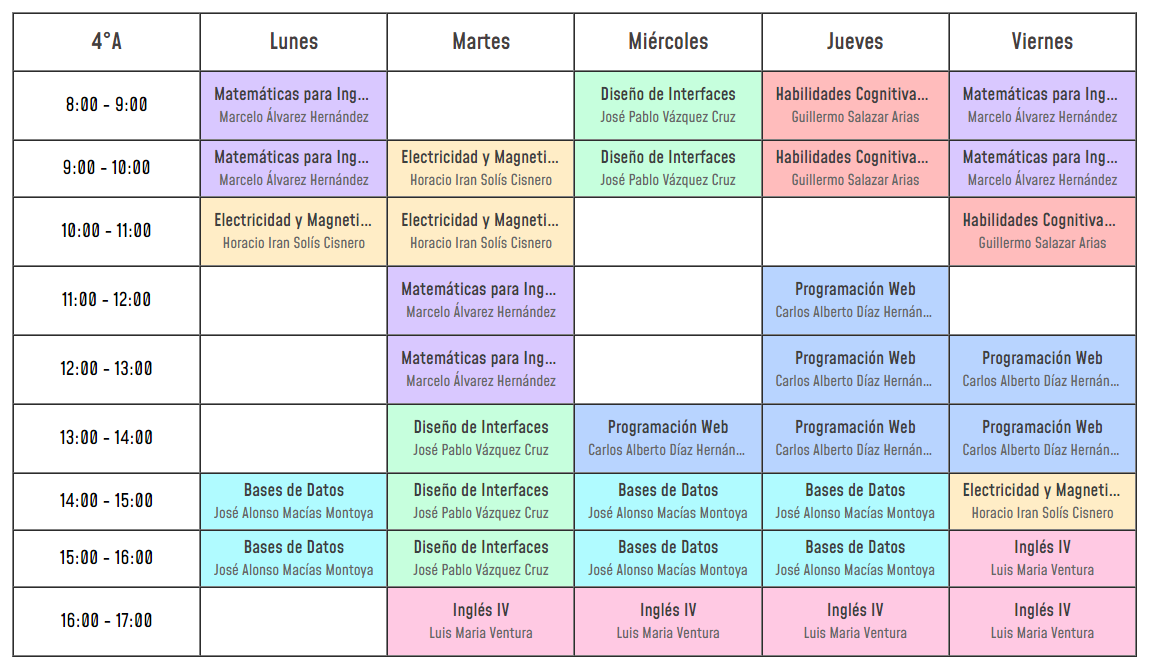
\includegraphics[width=0.7\textwidth]{images/available-groups.png}
    \caption{Horario del grupo disponible 4°A en el periodo Enero-Abril de 2024.}
    \label{fig:horario_del_grupo_disponible_4A_en_el_periodo_enero_abril_de_2024}
\end{figure}

Hemos asignado colores para cada materia perteneciente a cada horario para identificar de una manera más sencilla la distribución de una materia.

\subsection{Resultado} \label{resultados}
Tras finalizar el algoritmo genético, y obtener los resultados, la aplicación web se encarga de mostrar el horario correspondiente a la mejor opción y meta dato como detalles de la semilla.

A diferencia de los calendarios de la figura \ref{fig:horario_del_grupo_disponible_4A_en_el_periodo_enero_abril_de_2024}, en este horario de resultado se muestra el grado y grupo de la materia en cada celda horaria.

\begin{figure}[h]
    \centering
    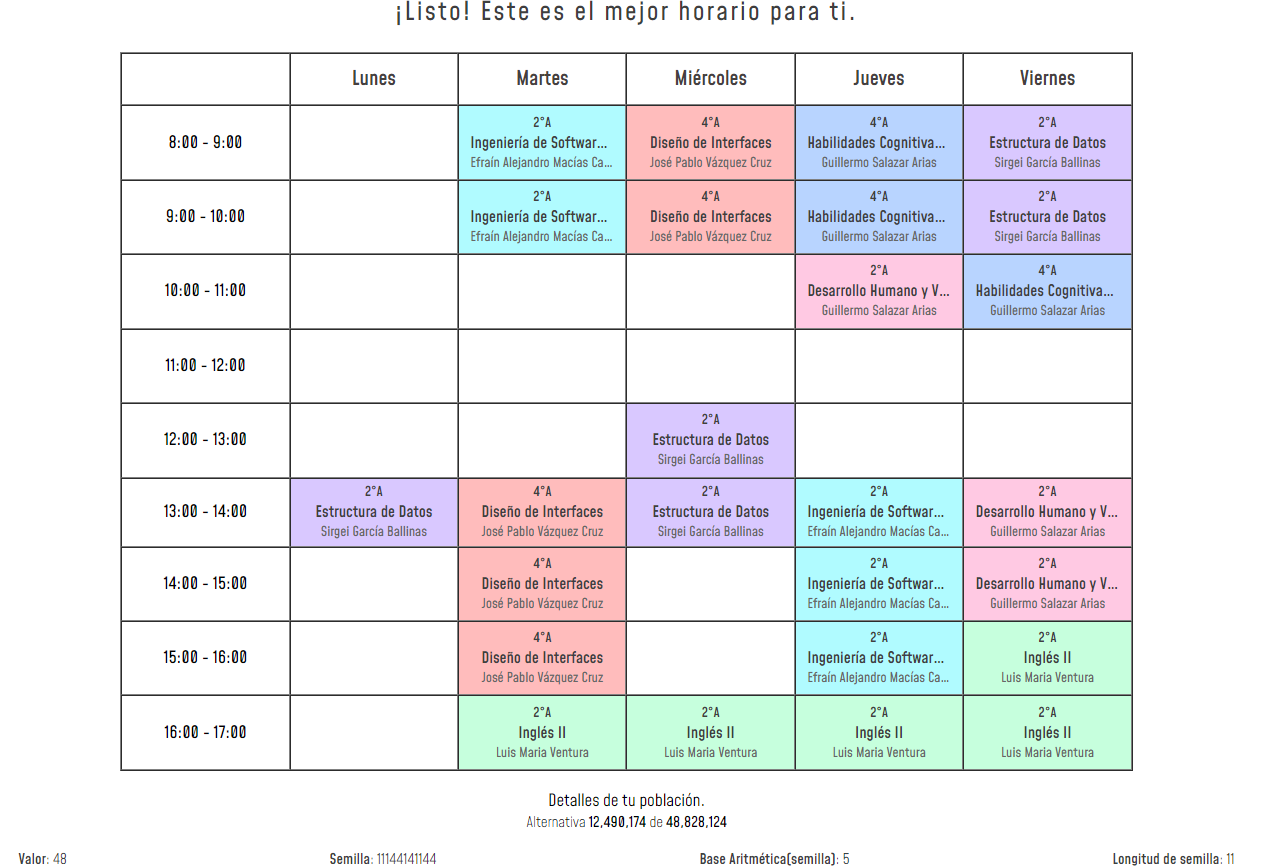
\includegraphics[width=\textwidth]{images/result.png}
    \caption{Resultado para la generación de horario de 1000 generaciones de la selección de la figura \ref{fig:seccion_de_seleccion_de_estado_actual_del_usuario}.}
    \label{fig:resultado}
\end{figure}

\subsection{Estadísticas} \label{estadisticas}
La parte estadística muestra la generación histórica a través de la \(n\) cantidad de generaciones definida por el usuario en opciones avanzadas.

Estas gráficas se muestran en la sección de resultado, justo de bajo del calendario óptimo (ver figura \ref{fig:resultado}), y muestra de forma visual, el mejor caso, que corresponde al individuo de mayor peso de dicha generación; el peor caso, que corresponde al individuo de menor peso de dicha generación; y promedio, que corresponde al peso promedio de todos los individuos calculados en dicha generación (incluyendo al mejor y peor caso).

Estas gráficas son generadas para los individuos sin colisiones y para los individuos históricos (incluyendo los individuos con colisiones) (ver sección \ref{individuos}).

Para la gráfica de los individuos sin colisiones (figura \ref{fig:statics_no_colision}), se preservan al mejor y al peor histórico, por lo que el mejor caso de la generación actual no es tomado en cuenta, al menos que supero al mejor caso histórico.

Para la gráfica de los indivuos con colisiones (figura \ref{fig:statics_colision}), se gráfican únicamente los mejores y peores casos de la generación actual, esto por temas de rendimiento.

\begin{figure}[h]
    \centering
    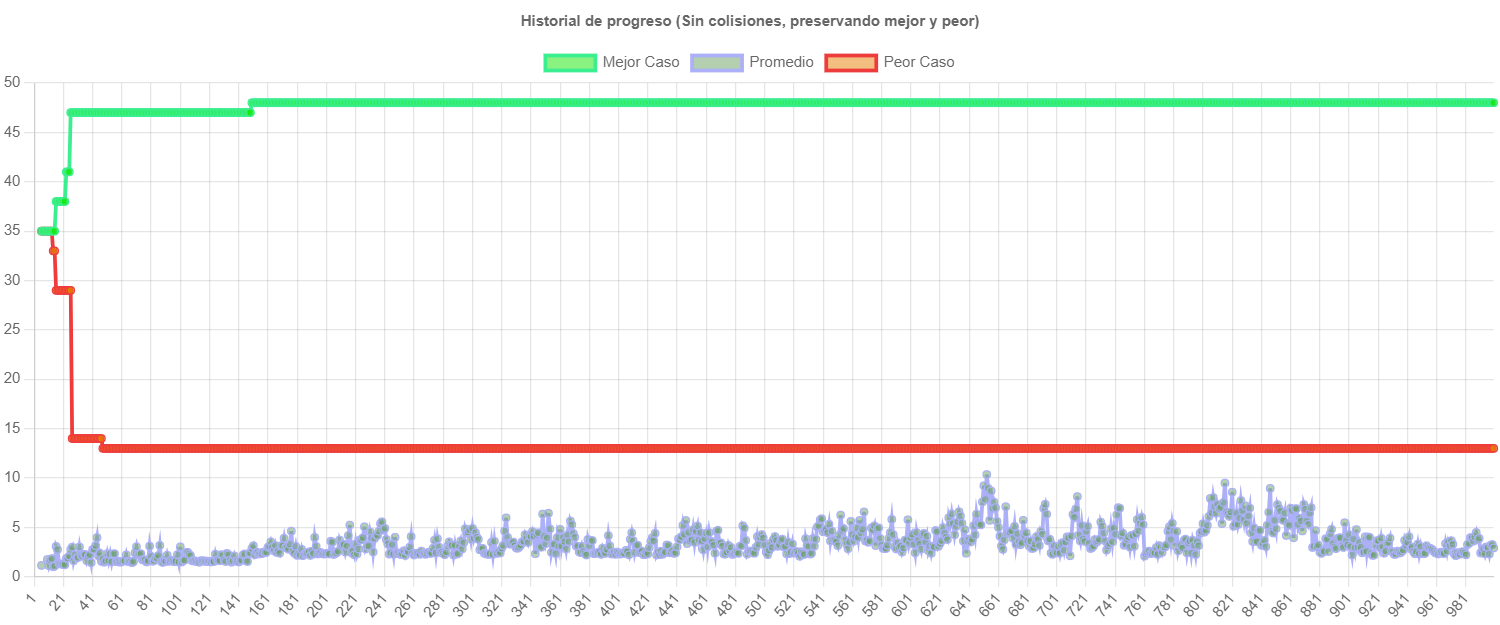
\includegraphics[width=0.9\textwidth]{images/no-colision.png}
    \caption{Estadadísticas historicas sin colisión de la de la selección de la figura \ref{fig:seccion_de_seleccion_de_estado_actual_del_usuario}, después mil generaciones}
    \label{fig:statics_no_colision}
\end{figure}

\begin{figure}[h]
    \centering
    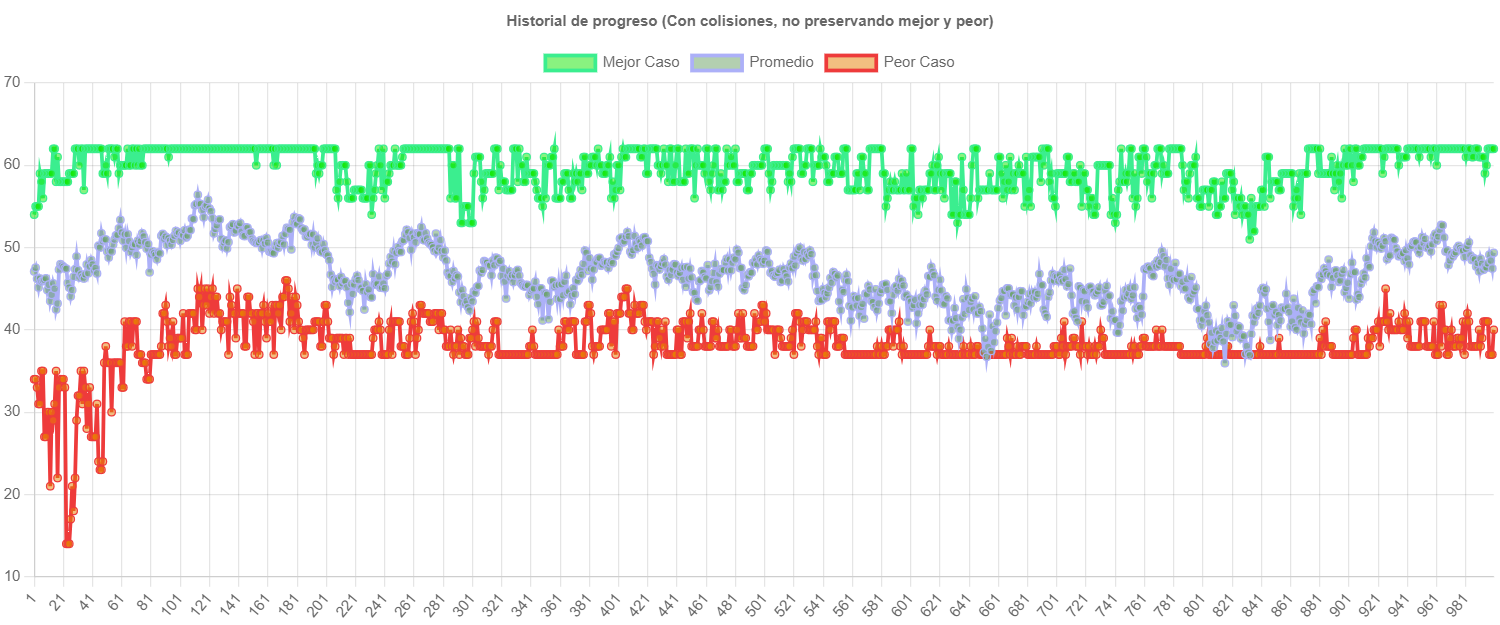
\includegraphics[width=0.9\textwidth]{images/with-colision.png}
    \caption{Estadadísticas historicas con colisión de la de la selección de la figura \ref{fig:seccion_de_seleccion_de_estado_actual_del_usuario}, después mil generaciones}
    \label{fig:statics_colision}
\end{figure}

\section{Herramientas} \label{herramientas}

En esta sección se detallan las herramientas utilizadas en el desarrollo de la aplicación, abarcando tanto el frontend como el backend, así como las tecnologías empleadas para el despliegue del servicio.

Para la interfaz de usuario de la aplicación, se empleó React JS, un framework de JavaScript ampliamente utilizado para la construcción de interfaces de usuario interactivas y eficientes. Además, se utilizó Chart.js para la visualización de gráficos web, lo que permitió representar de manera clara y concisa la información generada por el algoritmo genético.

En el lado del servidor, se utilizó Flask, un framework de Python para el desarrollo de aplicaciones web, junto con Python para la implementación del algoritmo genético. Para exponer el servicio del algoritmo genético, se optó por utilizar Waitress, un servidor web WSGI de Python que proporciona un equilibrio entre simplicidad y rendimiento, siendo adecuado para entornos de producción.

Además, para mejorar el rendimiento y tiempo de carga de la aplicación, se optó por implementar ciertas funcionalidades de manera nativa en Python, aprovechando su potencial en términos de procesamiento de datos y eficiencia.

Finalmente, para orquestar el lanzamiento del servicio en Waitress y el build de React servido con la imagen de Nginx, se empleó Docker Compose, una herramienta que permite definir y ejecutar aplicaciones Docker multi-contenedor de forma sencilla y eficiente. Esto facilitó la ejecuión y la gestión de la aplicación en diferentes entornos de desarrollo y producción.


\section{Conclusión}

El algoritmo genético diseñado y presentado en este documento ofrece una solución innovadora y eficaz para abordar la problemática de la selección óptima de materias en un contexto de irregularidad académica. Al considerar tanto los grupos disponibles en el cuatrimestre próximo como la secuencia recomendada dentro del plan de estudios y el progreso académico del estudiante, esta herramienta de software proporciona una distribución más adecuada de las materias, facilitando así la toma de decisiones informadas por parte de los estudiantes.

La exposición detallada del análisis realizado, la metodología empleada y el desarrollo del software en este documento no solo brinda una comprensión clara del funcionamiento del algoritmo genético, sino que también destaca su aplicación práctica y su relevancia en el contexto educativo actual. Se espera que esta herramienta proporcione un apoyo valioso a los estudiantes y administradores educativos al optimizar el proceso de selección de materias y mejorar la eficiencia académica en general.
